\documentclass{article}
\usepackage{hyperref}
\usepackage{graphicx}
\usepackage{float}


\title{Simple Document}
\author{Jakub Śliwka}
\date{03 March 2022}

\begin{document}

\maketitle

\section{First Section}

Later, it was said the man came from the north, from Ropers Gate. He came
on foot, leading his laden horse by the bridle. It was late afternoon and the
ropers’, saddlers’ and tanners’ stalls were already closed, the street empty. It
was hot but the man had a black coat thrown over his shoulders. He drew
attention to himself.
He stopped in front of the Old Narakort Inn, stood there for a moment,
listened to the hubbub of voices. As usual, at this hour, it was full of people.
The stranger did not enter the Old Narakort. He pulled his horse farther
down the street to another tavern, a smaller one, called The Fox. Not
enjoying the best of reputations, it was almost empty.
The innkeeper raised his head above a barrel of pickled cucumbers and
measured the man with his gaze. The outsider, still in his coat, stood stiffly
in front of the counter, motionless and silent.
"What will it be?"
"Beer," said the stranger. His voice was unpleasant.
The innkeeper wiped his hands on his canvas apron and filled a chipped
earthenware tankard.
The stranger was not old but his hair was almost entirely white. Beneath
his coat he wore a worn leather jerkin laced up at the neck and shoulders.
As he took off his coat those around him noticed that he carried a sword
—not something unusual in itself, nearly every man in Wyzim carried a
weapon—but no one carried a sword strapped to his back as if it were a
bow or a quiver.
The stranger did not sit at the table with the few other guests. He
remained standing at the counter, piercing the innkeeper with his gaze. He
drew from the tankard.
"I’m looking for a room for the night."
"There's none," grunted the innkeeper, looking at the guest's boots, dusty
and dirty. "Ask at the Old Narakort."
"I would rather stay here."
"There is none." The innkeeper finally recognized the stranger's accent.
He was Rivian.
"I’ll pay." 

\subsection{First Subsection}
\subsubsection{First Subsubsection}

\section{Text Styles}
This text is written in \textit{italic}, this text is \underline{underlined}, this text is \textbf{bold} and this \textbf{\textit{\underline{has everything}}}.

\section{Environments}
\subsection{Lists}
Unordered lists
\begin{itemize}
    \item this
    \item is
    \item a 
    \item list
\end{itemize}
Ordered lists
\begin{enumerate}
    \item this
    \item is
    \item a 
    \item list
\end{enumerate}

\subsection{Equations}
We have inline equations, e.g., the delta equation is $\Delta=b^2-4ac$, but we also have full equations, that we like:
\begin{equation}
    \label{eq_sum}
    \sum_{n=1}^{4} n = 1 + 2 + 3 + 4 = 10 
\end{equation}

Comment to (\ref{eq_sum}) equation
\begin{equation}
    \int_{a}^b f(x)dx = tmp_text
    \label{eq_integral}
\end{equation}

Comment to (\ref{eq_integral}) equation

\section{Tables}

\begin{table}[H]
    \centering
    \begin{tabular}{|l|c|r|}
    \hline
    Column A with Data & Column C with Data & \textbf{Column C with Data} \\ \hline
    data 1             & data 3             & \textbf{data 5}             \\ \hline
    data 2             & data 4             & \textbf{data 6}             \\ \hline
    \end{tabular}
    \caption{Table nr 1}
\end{table}
Example table generator: \url{https://www.tablesgenerator.com/}

\section{Images}
\LaTeX\ allows easy inclusion of images in the document.

\begin{figure}[htbp]
    \centering
    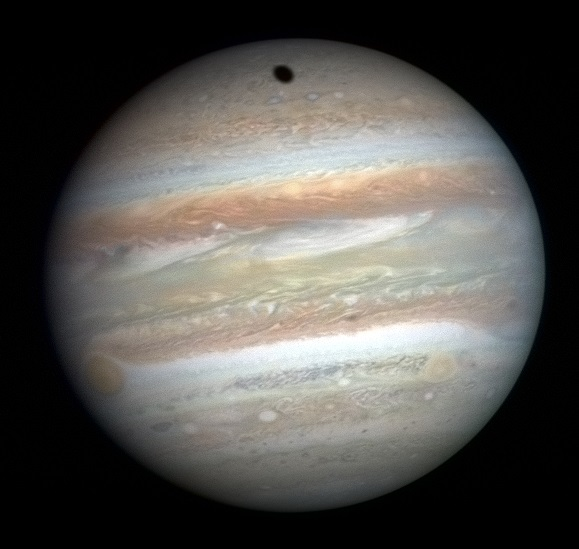
\includegraphics[scale=0.3]{Jupiter_New_Horizons.jpg}
    \caption{Jupiter or something idk [\ref{jupiter}]}
    \label{jupiter}
\end{figure}

\begin{thebibliography}{9}
    \bibitem{jupiterb}
    en.wikipedia.org  \emph{Jupiter New Horizons}
    Accessed: 04 MArch, 2024.
\end{thebibliography}

\end{document}
